% !TEX spellcheck = en_US



% ~~~~~~~~~~~~~~~~~~~~~~~~~~~~~~~~~~~~~~~ V
% (NC) 2026 Haluk Bingol
% github.com/halukbingol/LaTeX-Templates
%
% Licensees may copy, distribute, display, and perform the work and make derivative works 
% and remixes based on it only for non-commercial purposes. 
% ~~~~~~~~~~~~~~~~~~~~~~~~~~~~~~~~~~~~~~~ A




% =====================================================================
%  Linked Lists -- Freshman Level
%  ---------------------------------------------------------------------
%  Built on hblib/Template/hblibTemplate.tex with the libraries in ../../hblib/.
%  Programs and their real outputs are in codeoutput/:
%     codeoutput/<Name>.java   a program (classes without main() are only compiled)
%     codeoutput/<Name>.txt    what it printed
%     codeoutput/Check.txt     a captured `java -version`
% =====================================================================

\documentclass[aspectratio=169,10pt,compress]{beamer}

% ~~~~~~~~~~~~~~~~~~~~~~~~~~~~~~~~~~~~~~~~~~~~~~~~~~~~~~~~~~~~~~~~~ V hblib
	\usepackage{../../hblib/hblibPresentation} % lib presentation: theme, i/N, \hSection, algorithm2e, ...
	\usepackage{../../hblib/hblibCodeoutput} % lib code + output: \lstcode, \lstterminal, ...
	\usepackage{../../hblib/hblibDatastructures} % lib data structures: \hString, \hStack, \hQueue
% ~~~~~~~~~~~~~~~~~~~~~~~~~~~~~~~~~~~~~~~~~~~~~~~~~~~~~~~~~~~~~~~~~ A hblib


\usepackage[T1]{fontenc}
\usepackage{lmodern}
\usepackage{booktabs}

\newcommand{\win}{\textbf{Windows}}
\newcommand{\mac}{\textbf{macOS}}

% long Java lines: wrap instead of running off the frame
\lstset{columns=fixed, breaklines=true, breakatwhitespace=false}

\SetAlCapFnt{\small}
\SetAlCapNameFnt{\small}
\SetKwProg{Fn}{function}{}{end}
\SetKw{KwError}{error}

% ---------------------------------------------------------------------
\title{Linked Lists}
\subtitle{Freshman Level: Your First Chain of Nodes}
\author[Alpaydin]{Ruhan Alpaydin}

\institute[FCIS]{
    Faculty of Computer and Information Sciences\\
    Yeditepe University
}
\date{
	{\tiny \hbTimeStamp}
}

\begin{document}




% ~~~~~~~~~~~~~~~~~~~~~~~~~~~~~~~~~~~~~~ V frm
\begin{frame}[t,fragile]
  \titlepage
\end{frame}
% ~~~~~~~~~~~~~~~~~~~~~~~~~~~~~~~~~~~~~~ A frm




% ~~~~~~~~~~~~~~~~~~~~~~~~~~~~~~~~~~~~~~ V frm
\begin{frame}[t,fragile] \frametitle{Outline}
  \begin{columns}[T]
    \begin{column}{0.48\textwidth}
      \tableofcontents[sections={1-3}, hideallsubsections]
    \end{column}
    \begin{column}{0.48\textwidth}
      \tableofcontents[sections={4-6}, hideallsubsections]
    \end{column}
  \end{columns}
\end{frame}
% ~~~~~~~~~~~~~~~~~~~~~~~~~~~~~~~~~~~~~~ A frm

% ~~~~~~~~~~~~~~~~~~~~~~~~~~~~~~~~~~~~~~ V
\hSection[Ready]{Getting Ready}
% ~~~~~~~~~~~~~~~~~~~~~~~~~~~~~~~~~~~~~~ A




% ~~~~~~~~~~~~~~~~~~~~~~~~~~~~~~~~~~~~~~ V frm
\begin{frame}[t,fragile] \frametitle{What you need}
  \begin{itemize}
    \item A \textbf{JDK} 17 or newer: it has \hCode{javac} (compiler) and \hCode{java} (runner).
    \item A terminal and a text editor (or an IDE such as Eclipse, IntelliJ IDEA).
    \item One folder for this week, e.g.\ \hCode{linkedlist}, with all \hCode{.java} files in it.
  \end{itemize}
  \begin{columns}[T]
    \begin{column}{0.48\textwidth}
      \begin{block}{Windows (Command Prompt)}
\begin{lstlisting}[style=codesnippet, language={}, basicstyle=\ttfamily\scriptsize]
winget install EclipseAdoptium.Temurin.21.JDK
rem open a NEW Command Prompt, then:
mkdir linkedlist
cd linkedlist
\end{lstlisting}
      \end{block}
    \end{column}
    \begin{column}{0.48\textwidth}
      \begin{block}{macOS (Terminal)}
\begin{lstlisting}[style=codesnippet, language=bash, basicstyle=\ttfamily\scriptsize]
brew install --cask temurin@21
# or the .pkg from adoptium.net
mkdir linkedlist
cd linkedlist
\end{lstlisting}
      \end{block}
    \end{column}
  \end{columns}
  \small Check with:
  \lstterminal[basicstyle=\ttfamily\scriptsize]{codeoutput/Check.txt}
\end{frame}
% ~~~~~~~~~~~~~~~~~~~~~~~~~~~~~~~~~~~~~~ A frm




% ~~~~~~~~~~~~~~~~~~~~~~~~~~~~~~~~~~~~~~ V frm
\begin{frame}[t,fragile] \frametitle{A linked list in one picture}
  \begin{center}
  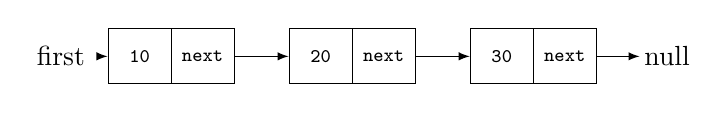
\begin{tikzpicture}
    \node at (-1.4,0) {\hCode{first}};
    \node[draw, minimum width=1.6cm, minimum height=0.7cm] (a) at (0,0) {};
    \node[font=\ttfamily\scriptsize] at (-0.4,0) {10};
    \node[font=\ttfamily\scriptsize] at ( 0.4,0) {next};
    \draw (a.north) -- (a.south);
    \node[draw, minimum width=1.6cm, minimum height=0.7cm] (b) at (2.3,0) {};
    \node[font=\ttfamily\scriptsize] at (1.9,0) {20};
    \node[font=\ttfamily\scriptsize] at (2.7,0) {next};
    \draw (b.north) -- (b.south);
    \node[draw, minimum width=1.6cm, minimum height=0.7cm] (c) at (4.6,0) {};
    \node[font=\ttfamily\scriptsize] at (4.2,0) {30};
    \node[font=\ttfamily\scriptsize] at (5.0,0) {next};
    \draw (c.north) -- (c.south);
    \node at (6.3,0) {\hCode{null}};
    \draw[-latex] (-0.85,0) -- (a.west);
    \draw[-latex] (a.east)  -- (b.west);
    \draw[-latex] (b.east)  -- (c.west);
    \draw[-latex] (c.east)  -- (5.95,0);
  \end{tikzpicture}
  \end{center}
  \vspace{0.4em}
  \begin{itemize}\small
    \item Each box is a \textbf{node}: a data value and a reference to the next node.
    \item The whole list is reached through one reference, \hCode{first}.
    \item The last node's \hCode{next} is \hCode{null}: that is how the chain ends.
    \item \hRemark{You cannot jump}. Every access starts at \hCode{first} and walks.
  \end{itemize}
\end{frame}
% ~~~~~~~~~~~~~~~~~~~~~~~~~~~~~~~~~~~~~~ A frm

% ~~~~~~~~~~~~~~~~~~~~~~~~~~~~~~~~~~~~~~ V
\hSection[Link]{The Link Class}
% ~~~~~~~~~~~~~~~~~~~~~~~~~~~~~~~~~~~~~~ A




% ~~~~~~~~~~~~~~~~~~~~~~~~~~~~~~~~~~~~~~ V frm
\begin{frame}[t,fragile] \frametitle{\texttt{Link}: three fields}
  \begin{columns}[T]
    \begin{column}{0.50\textwidth}
      \lstcode[basicstyle=\ttfamily\scriptsize]{codeoutput/Link.java}{Java}
    \end{column}
    \begin{column}{0.46\textwidth}
      \begin{itemize}\small
        \item \hCode{iData}, \hCode{dData}: the payload.
        \item \hCode{next}: the reference to the next node, or \hCode{null}.
        \item The constructor leaves \hCode{next} at \hCode{null} by default.
        \item \hCode{displayLink} prints one node as \hCode{[iData, dData]}.
      \end{itemize}
    \end{column}
  \end{columns}
\end{frame}
% ~~~~~~~~~~~~~~~~~~~~~~~~~~~~~~~~~~~~~~ A frm

% ~~~~~~~~~~~~~~~~~~~~~~~~~~~~~~~~~~~~~~ V
\hSection[List]{The LinkList Class}
% ~~~~~~~~~~~~~~~~~~~~~~~~~~~~~~~~~~~~~~ A




% ~~~~~~~~~~~~~~~~~~~~~~~~~~~~~~~~~~~~~~ V frm
\begin{frame}[t,fragile] \frametitle{\texttt{LinkList}: \texttt{insertFirst}}
  \begin{columns}[T]
    \begin{column}{0.50\textwidth}
      \lstcode[basicstyle=\ttfamily\scriptsize, firstline=6, lastline=10, firstnumber=6]{codeoutput/LinkList.java}{Java}
    \end{column}
    \begin{column}{0.46\textwidth}
      \begin{block}{Two references change}
        \small
        1. the new node's \hCode{next} $\gets$ the old \hCode{first};\\
        2. \hCode{first} $\gets$ the new node.
      \end{block}
      \begin{block}{Cost}
        \small
        Two assignments, no loop. \hRemark{$O(1)$}.
      \end{block}
    \end{column}
  \end{columns}
\end{frame}
% ~~~~~~~~~~~~~~~~~~~~~~~~~~~~~~~~~~~~~~ A frm




% ~~~~~~~~~~~~~~~~~~~~~~~~~~~~~~~~~~~~~~ V frm
\begin{frame}[t,fragile] \frametitle{\texttt{LinkList}: \texttt{deleteFirst}}
  \begin{columns}[T]
    \begin{column}{0.50\textwidth}
      \lstcode[basicstyle=\ttfamily\scriptsize, firstline=12, lastline=17, firstnumber=12]{codeoutput/LinkList.java}{Java}
    \end{column}
    \begin{column}{0.46\textwidth}
      \begin{block}{Three statements}
        \small
        1. save the old \hCode{first};\\
        2. advance \hCode{first} to \hCode{first.next};\\
        3. return the saved node.
      \end{block}
      \begin{block}{Edge case}
        \small
        Empty list: return \hCode{null}, do not crash. \hRemark{$O(1)$}.
      \end{block}
    \end{column}
  \end{columns}
\end{frame}
% ~~~~~~~~~~~~~~~~~~~~~~~~~~~~~~~~~~~~~~ A frm




% ~~~~~~~~~~~~~~~~~~~~~~~~~~~~~~~~~~~~~~ V frm
\begin{frame}[t,fragile] \frametitle{\texttt{LinkList}: \texttt{displayList}}
  \begin{columns}[T]
    \begin{column}{0.50\textwidth}
      \lstcode[basicstyle=\ttfamily\scriptsize, firstline=19, lastline=24, firstnumber=19]{codeoutput/LinkList.java}{Java}
    \end{column}
    \begin{column}{0.46\textwidth}
      \begin{itemize}\small
        \item A \hCode{for} loop starting at \hCode{first},
              following \hCode{next} until \hCode{null}.
        \item The condition \hCode{current != null} stops the walk at
              the end of the chain.
        \item \hRemark{Every traversal of a linked list has this shape}.
      \end{itemize}
    \end{column}
  \end{columns}
\end{frame}
% ~~~~~~~~~~~~~~~~~~~~~~~~~~~~~~~~~~~~~~ A frm




% ~~~~~~~~~~~~~~~~~~~~~~~~~~~~~~~~~~~~~~ V frm
\begin{frame}[t,fragile] \frametitle{\texttt{LinkList}: \texttt{find}}
  \begin{columns}[T]
    \begin{column}{0.50\textwidth}
      \lstcode[basicstyle=\ttfamily\scriptsize, firstline=26, lastline=30, firstnumber=26]{codeoutput/LinkList.java}{Java}
    \end{column}
    \begin{column}{0.46\textwidth}
      \begin{itemize}\small
        \item Same loop shape as \hCode{displayList}.
        \item Inside the loop, test the key: if it matches, return the node.
        \item If the loop ends, the key is not in the list: return \hCode{null}.
        \item \hRemark{$O(n)$}: the only search is a walk.
      \end{itemize}
    \end{column}
  \end{columns}
\end{frame}
% ~~~~~~~~~~~~~~~~~~~~~~~~~~~~~~~~~~~~~~ A frm




% ~~~~~~~~~~~~~~~~~~~~~~~~~~~~~~~~~~~~~~ V frm
\begin{frame}[t,fragile] \frametitle{\texttt{LinkList}: \texttt{delete}}
  \begin{columns}[T]
    \begin{column}{0.50\textwidth}
      \lstcode[basicstyle=\ttfamily\scriptsize, firstline=32, lastline=44, firstnumber=32]{codeoutput/LinkList.java}{Java}
    \end{column}
    \begin{column}{0.46\textwidth}
      \begin{block}{The two-pointer walk}
        \small
        \hCode{current} walks the chain; \hCode{previous} trails one
        node behind. When \hCode{current.iData == key}, you are ready
        to unlink.
      \end{block}
      \begin{block}{Two cases}
        \small
        \begin{itemize}
          \item \hCode{previous == null}: the match is at the head, so
                \hCode{first} moves.
          \item \hCode{previous != null}: \hCode{previous.next} skips
                over \hCode{current}.
        \end{itemize}
      \end{block}
    \end{column}
  \end{columns}
\end{frame}
% ~~~~~~~~~~~~~~~~~~~~~~~~~~~~~~~~~~~~~~ A frm

% ~~~~~~~~~~~~~~~~~~~~~~~~~~~~~~~~~~~~~~ V
\hSection[FirstLast]{FirstLastList}
% ~~~~~~~~~~~~~~~~~~~~~~~~~~~~~~~~~~~~~~ A




% ~~~~~~~~~~~~~~~~~~~~~~~~~~~~~~~~~~~~~~ V frm
\begin{frame}[t,fragile] \frametitle{\texttt{FirstLastList}: first and last}
  \begin{columns}[T]
    \begin{column}{0.50\textwidth}
      \lstcode[basicstyle=\ttfamily\scriptsize]{codeoutput/FirstLastList.java}{Java}
    \end{column}
    \begin{column}{0.46\textwidth}
      \lstterminal[basicstyle=\ttfamily\scriptsize]{codeoutput/FirstLastList.txt}
      \small
      A second reference, \hCode{last}, points at the tail.
      \hCode{insertLast} becomes $O(1)$: no walk required. That difference
      is the whole reason for the class.
    \end{column}
  \end{columns}
\end{frame}
% ~~~~~~~~~~~~~~~~~~~~~~~~~~~~~~~~~~~~~~ A frm

% ~~~~~~~~~~~~~~~~~~~~~~~~~~~~~~~~~~~~~~ V
\hSection[Mistakes]{Common Mistakes}
% ~~~~~~~~~~~~~~~~~~~~~~~~~~~~~~~~~~~~~~ A




% ~~~~~~~~~~~~~~~~~~~~~~~~~~~~~~~~~~~~~~ V frm
\begin{frame}[t,fragile] \frametitle{Mistake 1: forgetting the null check}
  \begin{columns}[T]
    \begin{column}{0.50\textwidth}
      \lstcode[basicstyle=\ttfamily\scriptsize]{codeoutput/Bug1.java}{Java}
    \end{column}
    \begin{column}{0.46\textwidth}
      \lstterminal[basicstyle=\ttfamily\scriptsize]{codeoutput/Bug1.txt}
      \small
      \hCode{top} is \hCode{null}; \hCode{top.item} dereferences it: NPE.
      The fix is a guard (\hCode{if (top == null) …}) or a \hCode{pop}
      that throws a named exception.
    \end{column}
  \end{columns}
\end{frame}
% ~~~~~~~~~~~~~~~~~~~~~~~~~~~~~~~~~~~~~~ A frm




% ~~~~~~~~~~~~~~~~~~~~~~~~~~~~~~~~~~~~~~ V frm
\begin{frame}[t,fragile] \frametitle{Mistake 2: forgetting \texttt{tail = null}}
  \begin{columns}[T]
    \begin{column}{0.50\textwidth}
      \lstcode[basicstyle=\ttfamily\scriptsize]{codeoutput/Bug2.java}{Java}
    \end{column}
    \begin{column}{0.46\textwidth}
      \lstterminal[basicstyle=\ttfamily\scriptsize]{codeoutput/Bug2.txt}
      \small
      After removing the only element, \hCode{head} is \hCode{null} but
      \hCode{tail} still points at it. The next \hCode{enqueue} chains
      from a node nothing can reach through \hCode{head}:
      \hRemark{the queue is broken}.
    \end{column}
  \end{columns}
\end{frame}
% ~~~~~~~~~~~~~~~~~~~~~~~~~~~~~~~~~~~~~~ A frm




% ~~~~~~~~~~~~~~~~~~~~~~~~~~~~~~~~~~~~~~ V frm
\begin{frame}[t,fragile] \frametitle{Mistake 3: wrong order in \texttt{insertFirst}}
  \begin{columns}[T]
    \begin{column}{0.50\textwidth}
      \lstcode[basicstyle=\ttfamily\scriptsize]{codeoutput/Bug3.java}{Java}
    \end{column}
    \begin{column}{0.46\textwidth}
      \lstterminal[basicstyle=\ttfamily\scriptsize]{codeoutput/Bug3.txt}
      \small
      \hCode{first = n} runs before \hCode{n.next = first}, so
      \hCode{n.next} becomes \hCode{n}. The list is one node pointing
      at itself: \hRemark{an infinite loop waiting to happen}.
    \end{column}
  \end{columns}
\end{frame}
% ~~~~~~~~~~~~~~~~~~~~~~~~~~~~~~~~~~~~~~ A frm




% ~~~~~~~~~~~~~~~~~~~~~~~~~~~~~~~~~~~~~~ V frm
\begin{frame}[t,fragile] \frametitle{Mistakes the compiler finds}
  \lstterminal[basicstyle=\ttfamily\scriptsize]{codeoutput/Typos.txt}
  \vspace{0.2em}
  \small
  Fix the \emph{first} error first. Java is \textbf{case sensitive}:
  \hCode{LinkList} is not \hCode{linklist}, and \hCode{java LinkList}
  is not \hCode{java linklist}.
\end{frame}
% ~~~~~~~~~~~~~~~~~~~~~~~~~~~~~~~~~~~~~~ A frm

% ~~~~~~~~~~~~~~~~~~~~~~~~~~~~~~~~~~~~~~ V
\hSection[Wrap]{Wrap-up}
% ~~~~~~~~~~~~~~~~~~~~~~~~~~~~~~~~~~~~~~ A




% ~~~~~~~~~~~~~~~~~~~~~~~~~~~~~~~~~~~~~~ V frm
\begin{frame}[t,fragile] \frametitle{First run: \texttt{LinkList} in action}
  \begin{columns}[T]
    \begin{column}{0.50\textwidth}
      \lstcode[basicstyle=\ttfamily\tiny]{codeoutput/LinkList.java}{Java}
    \end{column}
    \begin{column}{0.46\textwidth}
      \lstterminal[basicstyle=\ttfamily\scriptsize]{codeoutput/LinkList.txt}
      \small
      \hCode{insertFirst} builds the list in reverse order;
      \hCode{find} succeeds on 2, fails on 9; \hCode{delete(2)}
      removes the interior node.
    \end{column}
  \end{columns}
\end{frame}
% ~~~~~~~~~~~~~~~~~~~~~~~~~~~~~~~~~~~~~~ A frm




% ~~~~~~~~~~~~~~~~~~~~~~~~~~~~~~~~~~~~~~ V frm
\begin{frame}[t,fragile] \frametitle{Cheat sheet}
  \begin{columns}[T]
    \begin{column}{0.54\textwidth}
      \begin{center}\scriptsize
      \begin{tabular}{@{}ll@{}}
        \toprule
        \textbf{Task}              & \textbf{Code} \\
        \midrule
        empty list                 & \hCode{first == null} \\
        add at head                & \hCode{newLink.next = first;} \\
                                   & \hCode{first = newLink;} \\
        remove at head             & \hCode{first = first.next;} \\
        walk                       & \hCode{for (Link p = first; p != null; p = p.next)} \\
        find                       & same walk, test \hCode{p.iData == key} \\
        delete interior            & two pointers, \hCode{previous.next = current.next} \\
        add at tail (with last)    & \hCode{last.next = newLink;} \\
                                   & \hCode{last = newLink;} \\
        \bottomrule
      \end{tabular}
      \end{center}
    \end{column}
    \begin{column}{0.42\textwidth}
      \begin{block}{Do}
        \scriptsize
        check \hCode{first == null} first; update \hCode{first} and
        \hCode{last} together when the list becomes empty;
        walk with \hCode{current != null}.
      \end{block}
      \begin{block}{Don't}
        \scriptsize
        forget the \hCode{next} update; forget \hCode{tail = null};
        assign \hCode{first} before linking the new node.
      \end{block}
    \end{column}
  \end{columns}
\end{frame}
% ~~~~~~~~~~~~~~~~~~~~~~~~~~~~~~~~~~~~~~ A frm




% ~~~~~~~~~~~~~~~~~~~~~~~~~~~~~~~~~~~~~~ V frm
\begin{frame}[t,fragile] \frametitle{Practice}
  \begin{enumerate}\small
    \item Add \hCode{insertLast} to \hCode{LinkList} by walking to the
          end. Compare the cost with \hCode{FirstLastList.insertLast}.
    \item Write \hCode{size()} as a walk from \hCode{first} to \hCode{null}.
          Why is it $O(n)$ and not $O(1)$?
    \item Add \hCode{find} by \hCode{dData} instead of \hCode{iData}.
    \item Use \hCode{LinkList} to reverse a string: push each character,
          then pop them.
    \item Fix \hCode{Bug1}, \hCode{Bug2}, \hCode{Bug3} and re-run them so
          the errors disappear.
    \item Rewrite \hCode{delete(key)} so it works when \hCode{first}
          itself is the match. Reuse the two-pointer walk.
  \end{enumerate}
\end{frame}
% ~~~~~~~~~~~~~~~~~~~~~~~~~~~~~~~~~~~~~~ A frm




% ~~~~~~~~~~~~~~~~~~~~~~~~~~~~~~~~~~~~~~ V frm
\begin{frame}[t,fragile] \frametitle{References}
  \begin{enumerate}\small
    \item Robert Lafore, \emph{Data Structures \& Algorithms in Java},
          2nd ed., Sams, 2002. (The \hCode{Link} / \hCode{LinkList}
          style reused in this deck.)
    \item Oracle, \emph{Java SE 21 API Specification}:
          \hCode{java.util.LinkedList},
          \hCode{java.util.List}.
    \item Oracle, \emph{The Java Tutorials: Trail: Collections}.
    \item Joshua Bloch, \emph{Effective Java}, 3rd ed., Addison-Wesley,
          2018. (Items on \hCode{equals}, \hCode{hashCode}, \hCode{toString}.)
    \item Herbert Schildt, \emph{Java: The Complete Reference},
          12th ed., McGraw-Hill, 2021.
  \end{enumerate}
\end{frame}
% ~~~~~~~~~~~~~~~~~~~~~~~~~~~~~~~~~~~~~~ A frm




% ~~~~~~~~~~~~~~~~~~~~~~~~~~~~~~~~~~~~~~ V frm
\begin{frame}[t,fragile]
  \begin{center}
    \vspace{4cm}
    \hRemark{\Huge Questions?}
  \end{center}
\end{frame}
% ~~~~~~~~~~~~~~~~~~~~~~~~~~~~~~~~~~~~~~ A frm




\end{document}